%----------------------------------------
% Preamble to set up the document
%----------------------------------------
\documentclass{article}

% set up packages (you shouldn't need to touch this)
\usepackage{graphicx}  % required to insert images
\usepackage{hyperref}  % for hyperlinks
\usepackage[svgnames]{xcolor}  % to change hyperlink colors
\colorlet{linkcolour}{DarkBlue}
\hypersetup{colorlinks=true, linkcolor=linkcolour, citecolor=linkcolour, urlcolor=linkcolour,}

% Margins
\topmargin=-0.45in
\evensidemargin=0in
\oddsidemargin=0in
\textwidth=6.5in
\textheight=9.0in
\headsep=0.25in

% use a sans serif font
\renewcommand{\familydefault}{\sfdefault}

%----------------------------------------
% Step 1: Edit the lecture title
%----------------------------------------
\title{
Lecture 1: Reproducibility, replication, etc. \\  % Lecture title
Modeling Social Data, Spring 2017 \\   % Course title
Columbia University                    % School
}

%----------------------------------------
% Step 2: Edit your name and the date
%----------------------------------------
\author{Sai Srujan Chinta}                     % Scribe's name
\date{February 22, 2019}                % Lecture date

\begin{document}

\maketitle


%----------------------------------------
% Step 3:
% Rename uni.tex to match your uni,
% edit the filename accordingly below,
% and put your notes in this file
%----------------------------------------
%----------------------------------------
% Write your notes here
%----------------------------------------

\section{Motivation}
This lecture deals with challenges related to reproduciblity and replicability of scientific studies. The later part of the lecture gives an introduction to statistics and the correct way to interpret statistics.\\
While evaluating research results as a consumer, it is important to think critically about the study and formulate an informed opinion about whether or not the study can be believed. Here are a few questions to ask regarding the study:
\begin{enumerate}
    \item Was the research honest?
    \item How important is the result of the research?
    \item How robust is the result to small changes?
    \item Will the result of the research stand the test of time?
    \item Is the result real or was the data manipulated in order to obtain this result?
\end{enumerate}
For the rest of the lecture, we will assume that researchers are honest, although there is clear evidence which suggests the contrary.\footnote{\url{https://en.wikipedia.org/wiki/List_of_scientific_misconduct_incidents}}
\section{Reproducibility}
A study is said to be reproducible if the same results are obtained as those mentioned in the study upon conducting an individual experiment using the same data and same analysis. There are several challenges related to reproducibility:
\begin{enumerate}
    \item Data and code are not available publicly most of the time. Speifically, getting data from private companies to recreate ML/AI experiments is difficult since all the data and infrastructure will be needed. It becomes more problematic when something like reinforcement learning needs to be verified.
    \item Sometimes, even when the code is available, it is difficult to understand it, which makes it difficult to run the code.
    \item A major reason for this difficulty in running the code stems from the complex software dependencies of the programs.
\end{enumerate}
However, recent efforts by researchers in the form of better software engineering practices is improving the situation:
\begin{enumerate}
    \item Literate Programming
    \item Automated Build Scripts
    \item Containers
\end{enumerate}
\section{Replicability}
Replicability seeks to answer the question: Will the result hold up with new data but the same analysis? \\
Real-life datasets tend to be very small and noise can dominate signal in small datasets. Even in the case of large-datasets, asking enough questions leads to overfitting. \\
For example. consider an experiment wherein every classroom in Columbia is split into two sides and the number of IPhones owned by each side of each classroom is counted. Eventually, a conclusion can be drawn that the side of the room has an effect on IPhone ownership (even though this is clearly false). A different version of the same experiment is to take one very big classroom and conduct the same experiment on that big classroom. It is possible to find a feature which perfectly classifies this particular classroom but will not work for other classrooms. \\
An open science collaboration based in Virginia re-conducted 100 psychological experiments to check for replicability. The results of this study can be summarised as follows:
\begin{enumerate}
    \item Out of the $97\%$ studies which reported significant results, only $36\%$ reported statistically significant results.
    \item Only 47\% of the original results were in the 95\% confidence interval.
    \item In short, this study concluded that only half of what we read can be trusted. 
\end{enumerate}

\begin{figure}[ht]
  \begin{center}
    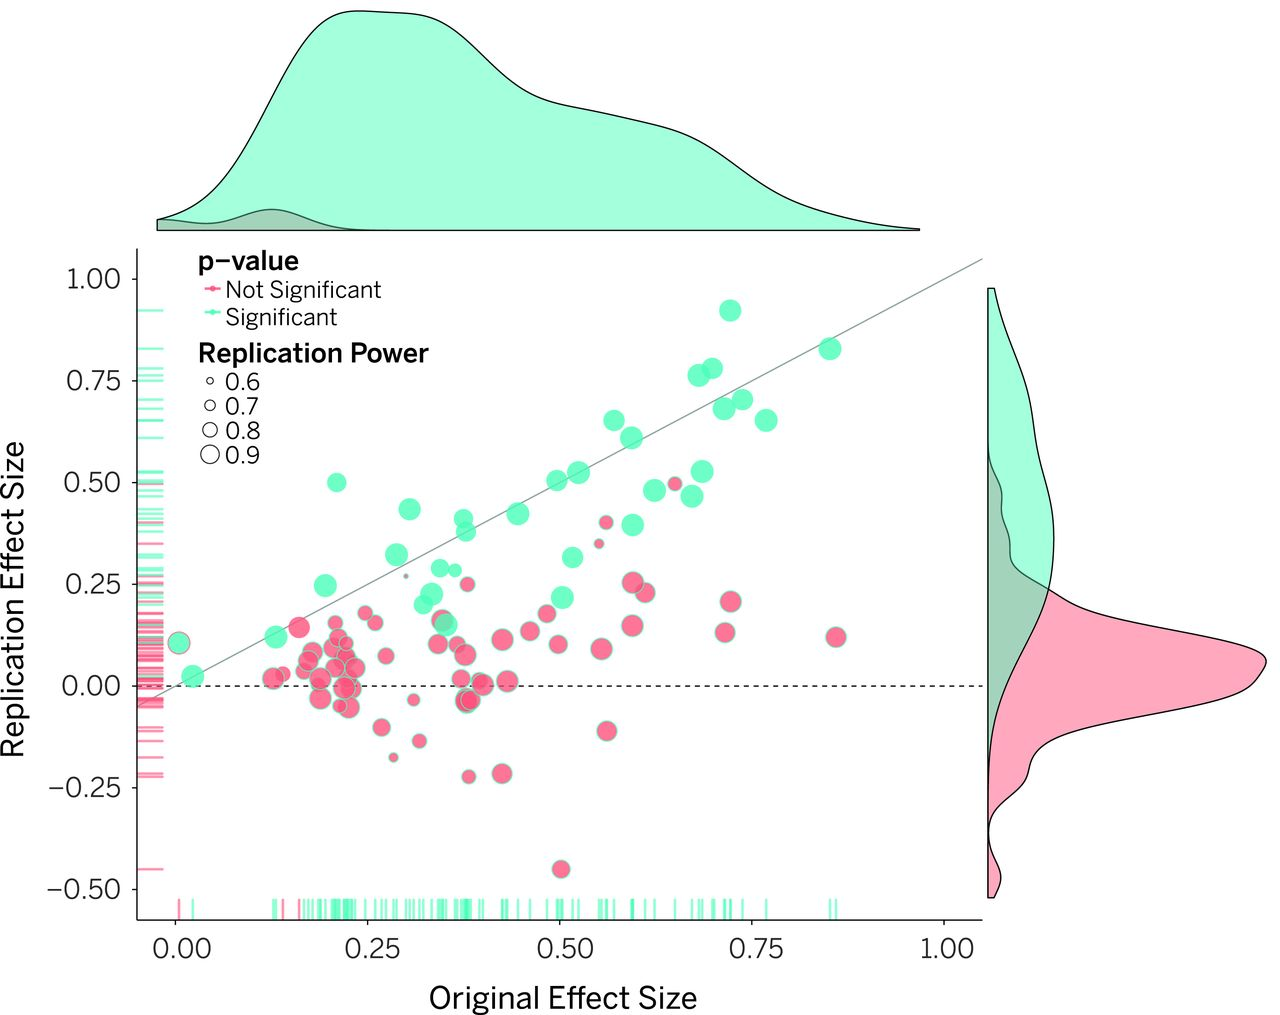
\includegraphics[width=0.5\textwidth,scale=2.0]{figures/replicationstudy.jpg}
    \caption{
      Original study effect size vs replication effect size}
    \label{fig:crisis}
  \end{center}
\end{figure}

Figure \ref{fig:crisis} is the result of the above mentioned experiment. The blue points along the diagonal represent perfect replicability. However, as can be seen in the figure \ref{fig:crisis}, there are far more red points than blue points and some experiments even resulted in negative correlation (replication study results directly contradict original study results).

\section{Statistics Quiz}
The answers and key take-aways of the quiz are as follows:
\begin{enumerate}
    \item Treatment A is preferred over Treatment B. To understand this answer, we must first understand the definition of standard error and how it relates to the sample size: 
    \begin{equation}
        \sigma_{se} = \frac{\sigma_{sd}}{\sqrt{n}}
    \end{equation}
    In the equation above, $\sigma_{sd}$ refers to the standard deviation in the population, $n$ refers to the sample size and $sigma_{se}$ refers to the standard deviation of the sampling distribution. In simple words, this equation tells us how uncertain we are about the mean. 
    \begin{figure}[ht]
      \begin{center}
        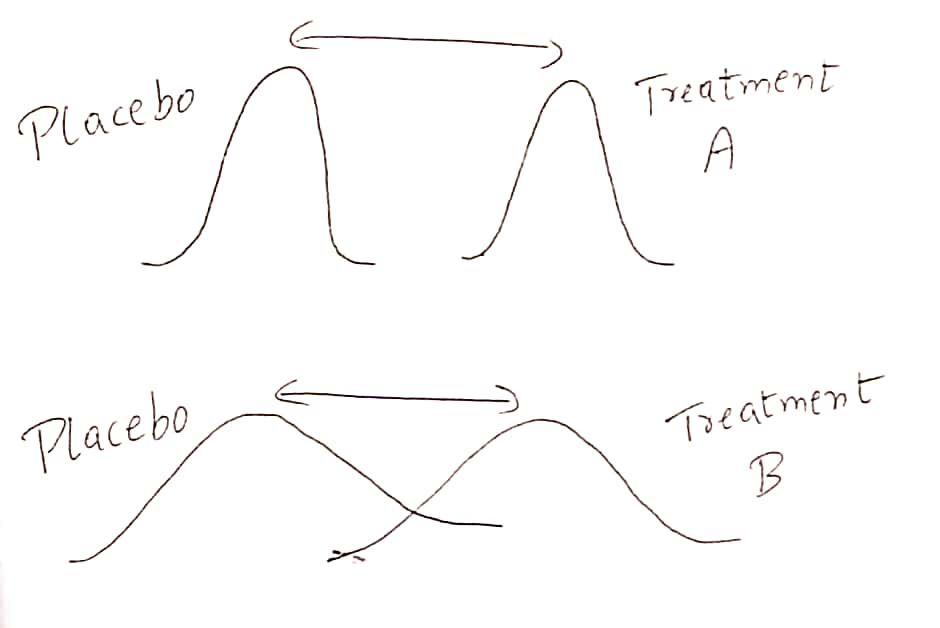
\includegraphics[width=0.5\textwidth,scale=2.0]{figures/msdq1.jpeg}
        \caption{
          Treatment A vs Treatment B}
        \label{fig:q1}
      \end{center}
    \end{figure}
    Therefore, though the mean separation is same in both the treatments, the population in Treatment A must have had lesser variance than that in Treatment B. If we plot out the effects of the placebo treatment and the effects of both Treatments A and B, the graph would look something like Figure \ref{fig:q1}. This graph clearly tells us that in some cases, the placebo performs better than Treatment B but this is never the case in Treatment A.
    \item All the statements are false. The reasons should become clear after reviewing the definition of p-value.
    \item The key take-away from this question is that data-visualisation can be used to mislead the readers and we should be wary of such attempts. The actual answer of the second part of this question is 57\% but the professor says that most people are willing to bet good money that the special boulder would slide farther than the normal one with a probability of upwards of 65\%.
\end{enumerate}
\section{Review of Statistics}
\begin{itemize}
    \item We cannot prove that theories are correct easily.
    \item Sometimes. we can find contradictions to prove things false.
    \item However, most of the time, we have to settle for ruling things out as "unlikely".
    \item We ask the question, "How unlikely are my results in a boring world?" (We will work with the assumption that when the null hypothesis $H_0$ is true, the world is boring)
    \item In practice, assume boring world ($H_0$ is true)
\end{itemize}
\begin{figure}[ht]
  \begin{center}
    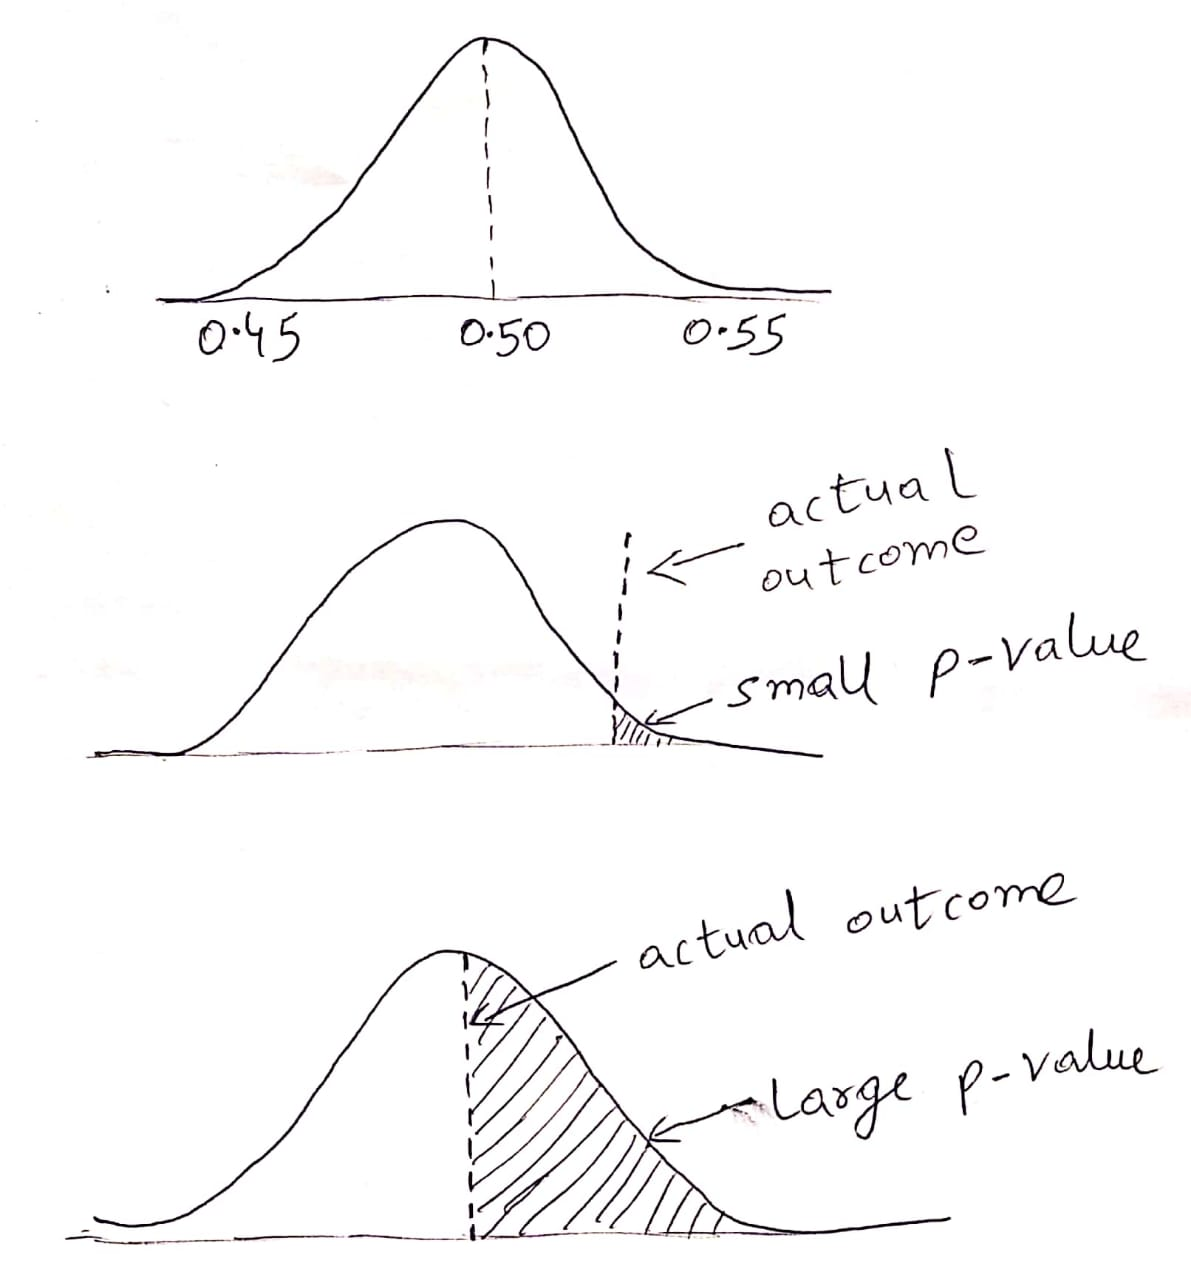
\includegraphics[width=0.5\textwidth,scale=2.0]{figures/pvalue.jpeg}
    \caption{
      Coin Toss Experiment}
    \label{fig:pvalue}
  \end{center}
\end{figure}
For example, let us consider the experiment wherein we toss a coin and try to find out if it is unbiased. For this experiment, we first take a fair coin (boring world) and toss it multiple times (say 100 times). We repeat this experiment (tossing a fair coin 100 times) multiple times and obtain the probabilities for each experiment. We can expect to see values like $p_0 = 0.52$, $p_0 = 0.48$ etc. However, when we plot these probabilities, we should obtain a normal distribution with the mean at around $p_0 = 0.5$. This normal distribution should look like the first figure in Figure \ref{fig:pvalue} We now take the actual coin which we wanted to test and toss it 100 times. We now plot the resulting probability in the normal distribution obtained from the boring world. If the resulting p-value is small, like the second figure in Figure \ref{fig:pvalue}, we reject the null hypothesis and conclude that the coin is biased. This is because the result we observed did not conform to the result we should have observed if our world was boring (if the coin was fair). However, if the resulting p-value is large, like the third figure in Figure \ref{fig:pvalue}, then we conclude that our world is boring and declare that the coin is fair. \\
Therefore, the p-value tells us the probability of data we observed we given that we are in a boring world (null hypothesis $H_0$ is true). \\
We also have to decide a threshold for the p-value below which we reject the boring world. This threshold is called the false positive rate $\alpha$. The convention is to pick $\alpha = 0.05$.\\
Power is defined as the probability of rejecting the null hypothesis $H_0$ given that it is false. In order to estimate this probability, we conduct the opposite experiment, i.e we assume an exciting world and run the experiment multiple times. Then, we compute the number of times we reject the null hypothesis and this results in Power. In order to correctly detect even small changes, i.e to be able to reject a boring world even with $p = 0.52$, we need huge sample size.

\end{document}

%%% Local Variables:
%%% mode: latex
%%% TeX-master: t
%%% End:
